% !TeX program = xelatex
% Chinese research manuscript using the Elsevier article class.
\documentclass[preprint,12pt]{elsarticle}
\usepackage[a4paper,margin=25mm]{geometry}
\usepackage[UTF8,fontset=none,scheme=plain]{ctex}
\usepackage{fontspec}
\IfFontExistsTF{Times New Roman}{\setmainfont{Times New Roman}}{\setmainfont{texgyretermes-regular.otf}[BoldFont=texgyretermes-bold.otf,ItalicFont=texgyretermes-italic.otf,BoldItalicFont=texgyretermes-bolditalic.otf]}
\IfFontExistsTF{SimSun}{\setCJKmainfont[AutoFakeBold=2,ItalicFont=SimSun,BoldItalicFont=SimSun]{SimSun}\setCJKmonofont{SimSun}}{\setCJKmainfont[BoldFont=FandolSong-Bold.otf,ItalicFont=FandolSong-Regular.otf,BoldItalicFont=FandolSong-Bold.otf]{FandolSong-Regular.otf}\setCJKmonofont{FandolSong-Regular.otf}}
\usepackage{amsmath,amssymb,unicode-math}
\setmathfont{latinmodern-math.otf}
\usepackage{etoolbox}
\usepackage{graphicx,booktabs,tabularx,array,caption,setspace,microtype,xurl,placeins}
\usepackage{needspace}
\biboptions{numbers,sort&compress}
\usepackage[hidelinks,unicode]{hyperref}
\hypersetup{pdftitle={BanG Dream国服活动排名分数的时序结构与活动条件关联},pdfauthor={Tano},pdfsubject={游戏数据观察性分析中文研究稿}}
\urlstyle{same}
\newcolumntype{L}{>{\raggedright\arraybackslash}X}
\newcolumntype{C}[1]{>{\centering\arraybackslash}p{#1}}
\captionsetup{font=small,labelfont=bf,justification=justified,singlelinecheck=false}
\renewcommand{\figurename}{图}
\renewcommand{\tablename}{表}
\renewcommand{\refname}{参考文献}
\abstracttitle{摘要}
\keywordtitle{\upshape 关键词}
\setstretch{1.15}
\setlength{\parindent}{2em}
\setlength{\parskip}{0.15em}
\setlength{\emergencystretch}{3em}
\hyphenpenalty=10000
\exhyphenpenalty=10000
\setlength{\textfloatsep}{12pt plus 2pt minus 2pt}
\setlength{\intextsep}{12pt plus 2pt minus 2pt}
\renewcommand{\topfraction}{0.92}
\renewcommand{\bottomfraction}{0.9}
\renewcommand{\textfraction}{0.05}
\renewcommand{\floatpagefraction}{0.8}
\setcounter{topnumber}{3}
\setcounter{totalnumber}{4}
\journal{Entertainment Computing}
% Show the manuscript page number without implying submission or acceptance.
\makeatletter
\patchcmd{\pprintMaketitle}{\vskip36pt}{\vskip12pt}{}{\errmessage{Title spacing patch failed}}
\def\ps@pprintTitle{\let\@oddhead\@empty\let\@evenhead\@empty
  \def\@oddfoot{\hfil\thepage\hfil}\let\@evenfoot\@oddfoot}
\makeatother
\newcommand{\NumEvents}{103}
\newcommand{\NumSourceCurves}{1\,871}
\newcommand{\NumValidCurves}{1\,780}
\newcommand{\NumPoints}{1\,796\,085}
\newcommand{\NumValidPoints}{1\,718\,910}
\newcommand{\NumExcluded}{91}
\newcommand{\NumCoreEvents}{94}
\newcommand{\NumCorrelationEvents}{92}
\newcommand{\PcaFirst}{90.573}
\newcommand{\PcaTwo}{96.523}
\newcommand{\NumCards}{2\,179}
\newcommand{\NumFiveStar}{346}
\newcommand{\NumCharacterMemberships}{527}
\newcommand{\NumTests}{26}
\newcommand{\NumNegativeAnchors}{125}
\newcommand{\NumAnchors}{23\,987}
\newcommand{\NumDecliningCurves}{48}
\newcommand{\NumDeclines}{50}
\newcommand{\SourceFingerprint}{c472560390f2}
\newcommand{\RhoFinal}{0.915}
\newcommand{\RhoGrowth}{0.471}
\newcommand{\RhoPartial}{0.736}
\newcommand{\CardBeta}{0.014}
\newcommand{\CardLower}{−0.030}
\newcommand{\CardUpper}{0.057}
\newcommand{\TimeBeta}{0.235}
\newcommand{\TimeLower}{0.158}
\newcommand{\TimeUpper}{0.313}
\newcommand{\DurationBeta}{1.231}
\newcommand{\DurationLower}{0.845}
\newcommand{\DurationUpper}{1.616}
\newcommand{\MygoBeta}{1.030}
\newcommand{\MygoLower}{0.707}
\newcommand{\MygoUpper}{1.352}
\newcommand{\ProgressEvents}{74}
\newcommand{\RemainingEvents}{86}
\newcommand{\HalfTop}{68.053}
\newcommand{\LateSixTop}{0.218}
\newcommand{\HalfThousand}{35.407}
\newcommand{\LateSixThousand}{19.360}
\newcommand{\HalfTwoThousand}{48.063}
\newcommand{\LateSixTwoThousand}{11.790}
\newcommand{\HalfThirtyThousand}{53.362}
\newcommand{\LateSixThirtyThousand}{4.419}
\newcommand{\RatioYearFirst}{1.707}
\newcommand{\RatioYearSecond}{2.515}
\newcommand{\RatioYearThird}{1.761}
\newcommand{\MatchedRareEvents}{15}
\newcommand{\InterpolationSix}{0.175}
\newcommand{\InterpolationQuarter}{1.030}

\clubpenalty=10000
\widowpenalty=10000
\displaywidowpenalty=10000
\begin{document}
\begin{frontmatter}
\title{BanG Dream国服活动排名分数的\\时序结构与活动条件关联}
\author{Tano}
\begin{abstract}
本文使用BanG Dream国服2024年1月29日起的\NumEvents{}期活动，分析19条排名线的分数分布、时间变化、末期增长及活动条件关联。数据快照包含\NumSourceCurves{}条曲线，其中\NumValidCurves{}条满足终点窗口要求。研究统一活动时间边界，分别使用成对可用样本和共同活动面板，并通过活动等权回归、活动聚类协方差及5期时间相关调整估计条件关联。在\NumCorrelationEvents{}期相同活动中，18线终分相关的中位数为\RhoFinal{}，半程剩余增长为\RhoGrowth{}；\NumCoreEvents{}期终分秩变量的第一主成分解释\PcaFirst{}\%方差。每年2月至10月的T1000/T2000终分比中位数依次为\RatioYearFirst{}、\RatioYearSecond{}和\RatioYearThird{}。共同\RemainingEvents{}期活动中，名义结束前6小时观测后的增长占终分中位数，T10为\LateSixTop{}\%，T1000为\LateSixThousand{}\%，T2000为\LateSixTwoThousand{}\%。活动类型和乐队与分数存在条件关联；加成角色近期卡牌发布数量的系数区间跨零。排名样本覆盖、采样分辨率和终点记录会影响汇总结果。现有数据支持区分共同分数水平、排名形状与阶段增长，相关结果的解释范围限于回溯性观察；玩家活跃人数、付费及个体投入有待其他数据测量。
\end{abstract}
\begin{keyword}
游戏数据分析 \sep 排名分数 \sep 时间结构 \sep 缺失覆盖 \sep 活动类型 \sep 乐队关联
\end{keyword}
\end{frontmatter}

\section*{Abstract}
{\raggedright\noindent\textbf{Temporal structure and event context associations in ranking scores from BanG Dream}\par}

We analyze ranking scores from \NumEvents{} events on the Chinese server of BanG Dream, covering 19 cutoffs from January 2024 onward. The snapshot contains \NumSourceCurves{} curves, of which \NumValidCurves{} satisfy the terminal observation window. Pairwise and common event panels separate score distributions, calendar changes, growth profiles, and context associations. Regression assigns equal total weight to each event and uses event cluster uncertainty with temporal adjustment. On the same \NumCorrelationEvents{} events, median correlations across 18 cutoffs are \RhoFinal{} for terminal scores and \RhoGrowth{} for remaining growth at the midpoint. In the complete panel of \NumCoreEvents{} events, the first principal component explains \PcaFirst{}\% of standardized terminal rank variance. Median ratios between the 1000th and 2000th cutoffs in matched months are \RatioYearFirst{}, \RatioYearSecond{}, and \RatioYearThird{} across 2024 to 2026. Growth after observations at six hours before the end varies substantially across cutoffs. Event type and band have conditional associations with scores, while the interval for recent card releases includes zero. Sampling resolution, missing coverage, and endpoint updates affect aggregate comparisons. These retrospective findings distinguish common score levels from ranking shape and growth. Individual effort, player counts, and spending require separate measurements.

\noindent\textbf{Keywords:} game analytics; ranking scores; temporal structure; missing data; event context

\section{引言}

限时排名活动将游戏中的得分过程汇总为随时间变化的榜线。对一场活动而言，T1000表示第1000名对应的分数，不同时刻占据该位置的玩家可以不同。因此，一条榜线同时包含活动整体分数水平、排名位置和阶段增长的信息。研究这些汇总数据，可以描述竞争分数的结构及其变化，但需要先明确可观测量和比较单位。

游戏数据分析通常从遥测记录中提取可重复的分布、时间模式与条件关联\citep{seif2013analytics,drachen2013mining}。公开榜线具有取得方便、时间跨度较长和多排名同步记录等特点，也有明显的测量限制：采样密度随排名变化，少数排名上线较晚，活动时长和规则类型不同，角色与乐队排程也随时间改变。这些条件会共同影响汇总统计。将来源不齐的终分中位数直接排列，可能把样本组成差异误读为排名结构；将分数水平的相关用于说明后续增长，也需要匹配相同活动重新检验。

本文围绕四个问题展开。第一，现有国服数据覆盖哪些活动和排名，其采样与终点质量如何。第二，各排名的分数水平和相对分数随时间怎样变化。第三，分数累积与末期增长在不同榜线之间有何差异。第四，在控制排名、时间和时长后，活动类型、乐队及近期卡牌发布与终分还存在怎样的关联。研究使用现有已结束活动的描述性快照，保留各指标的活动名单与来源指纹，并以共同面板检查覆盖差异的影响。

本文的分析对象为活动排名汇总分数。活跃人数、玩家持卡、游玩时长和付费记录属于未观测变量；这些变量需要单独的数据来源。文中使用“分数水平”和“后续增长”描述观测结果，避免将榜线直接换算为游戏总体规模或个体投入。

\section{数据来源与质量控制}

\subsection{来源、时间范围与统计单位}

活动、排名和内容元数据来自Bestdori公开数据\citep{bestdori2026}。本次于2026年11月18日从持续预测系统的线上运行库只读提取快照。活动按国服实际开始和结束时间筛选，要求实际开始时间不早于2024年1月29日13时，且在快照提取时已经结束。该时期采用密集采样，来源包含\NumEvents{}期活动，实际开始日期截至2026年11月5日，最后一期结束于2026年11月11日。尚在进行的活动不进入终分分析。

记录的基本单位为活动与排名对应的一条曲线。排名包括T10、T20、T30、T40、T50、T100、T200、T300、T400、T500、T1000、T1500、T2000、T3000、T4000、T5000、T10000、T20000和T30000。快照中的\NumSourceCurves{}条曲线保存\NumPoints{}个已归一化观测。每条曲线包含毫秒时间戳及以EP计的排名分数。活动ID用于连接记录，筛选与排序均依据实际时间。

活动元数据包含规则类型和加成角色列表；角色通过所属乐队映射为乐队构成。卡牌使用国服发布时间过滤，活动开始后发布的卡牌不计入该期可用内容。事件、角色与乐队缓存具有更新记录，卡牌缓存的历史内容与早期归档共同核对。各文件在快照中的字节哈希、采集状态和SQL条件随补充材料提供。回溯元数据保留了当前记录的历史属性，完整的历史时点版本仍有缺失。

\begin{table}[!htbp]
\centering\small
\caption{数据快照与分析范围}\label{tab:cohort}
\setlength{\tabcolsep}{4pt}
\renewcommand{\arraystretch}{1.15}
\begin{tabularx}{\linewidth}{l L}
\toprule
项目 & 数值或范围 \\
\midrule
数据采集区域 & 国服；服务器索引3 \\
活动实际开始日期 & 2024年1月29日至2026年11月5日 \\
最后活动结束时间 & 2026年11月11日22:59:59（UTC+8） \\
已结束活动／排名线 & \NumEvents{}／19 \\
存储曲线／合格曲线 & \NumSourceCurves{}／\NumValidCurves{} \\
存储观测／合格曲线内观测 & \NumPoints{}／\NumValidPoints{} \\
终点窗口未覆盖曲线 & \NumExcluded{} \\
活动类型／单乐队类别／混合乐队活动 & 6／8／28 \\
观测到的加成角色／角色与活动成员关系 & 40／\NumCharacterMemberships{} \\
18线共同终分／共同半程增长活动 & \NumCoreEvents{}／\NumCorrelationEvents{} \\
\bottomrule
\end{tabularx}
\par\vspace{4pt}
\begin{minipage}{\linewidth}\footnotesize\setstretch{1.05}
注：快照于2026年11月18日从线上运行库只读提取。观测数为库中已归一化的榜线记录；每条曲线对应一个活动与一个排名。
\end{minipage}
\end{table}


\subsection{终点窗口与曲线清理}

设活动开始和结束时刻为\(S_e\)与\(E_e\)，排名\(r\)的观测为\((u_{e,r,k},x_{e,r,k})\)。统一截取结束后5分钟以内的记录，以窗口内末次观测作为终分：
\begin{equation}\label{eq:terminal}
\begin{aligned}
k^*&=\arg\max_k\{u_{e,r,k}:u_{e,r,k}\leq E_e+5\ \mathrm{min}\},\\
Y_{e,r}&=x_{e,r,k^*},\qquad
u_{e,r,k^*}\geq E_e-1\ \mathrm{min}.
\end{aligned}
\end{equation}
同时要求活动时长为正，曲线至少含5个有效观测，终分大于零。无效数值和活动开始前的记录单独计数；相同时间戳按原记录顺序保留末项。本次快照未发现重复时间戳或无效数值。

按式~\eqref{eq:terminal}，\NumValidCurves{}条曲线满足终点要求，包含\NumValidPoints{}个观测；其余\NumExcluded{}条在规定窗口内缺少终点。每期至少有一条合格曲线，但各排名覆盖不同。另一个早期数据库保留了活动结束后的持续轮询，截取窗口后共排除210443个过晚采集点；线上库已执行相应的时间归一化。该采集差异记录在来源核查表中。

合格曲线中有\NumDecliningCurves{}条出现过分数下降，共\NumDeclines{}次。分析保留这些观测，未将曲线强制变为单调。终分与名义时点分数比较时，\NumAnchors{}个对齐记录中有\NumNegativeAnchors{}个产生负的后续增长。此类值提示榜线修订或采集过程的影响，具体原因需要回查接口记录。对同活动已观测的相邻排名终分，本次未发现排名顺序倒置。

\subsection{采样分辨率与缺失覆盖}

表~\ref{tab:ranks}和图~\ref{fig:sampling}展示19档的覆盖与间隔。T10以接近分钟的分辨率记录，其余多数档位接近30分钟。典型间隔先在每条曲线内部计算，再跨该档活动取中位数。较多采样点增加时间分辨率，但有效独立样本仍按活动计数。

\begin{table}[!htbp]
\centering\small
\caption{19条排名线的终分覆盖、分布与采样间隔}\label{tab:ranks}
\setlength{\tabcolsep}{4pt}
\renewcommand{\arraystretch}{1.15}
\begin{tabularx}{\linewidth}{l r r r L r}
\toprule
排名 & 源曲线 & 有效活动 & \shortstack{终分中位数\\/ 万EP} & 四分位范围 / 万EP & \shortstack{间隔中位数\\/ min} \\
\midrule
T10 & 103 & 99 & 5450.000 & [3631.556，8016.052] & 1.10 \\
T20 & 103 & 98 & 3441.148 & [2176.655，5250.000] & 30.03 \\
T30 & 103 & 98 & 2413.714 & [1650.511，3911.677] & 30.03 \\
T40 & 103 & 98 & 1983.368 & [1315.123，3225.893] & 30.03 \\
T50 & 103 & 98 & 1828.503 & [1221.971，3019.322] & 30.03 \\
T100 & 103 & 98 & 1338.612 & [797.736，2129.889] & 30.03 \\
T200 & 103 & 98 & 727.849 & [408.275，1256.258] & 30.03 \\
T300 & 103 & 98 & 612.665 & [347.310，1101.467] & 30.03 \\
T400 & 103 & 98 & 559.669 & [315.907，1067.232] & 30.03 \\
T500 & 103 & 98 & 550.991 & [297.758，1032.432] & 30.03 \\
T1000 & 103 & 98 & 448.074 & [259.777，916.825] & 30.03 \\
T1500 & 17 & 15 & 402.841 & [275.309，759.592] & 30.03 \\
T2000 & 103 & 98 & 235.863 & [138.415，356.936] & 30.03 \\
T3000 & 103 & 98 & 161.937 & [100.135，259.790] & 30.03 \\
T4000 & 103 & 98 & 131.273 & [84.655，225.181] & 30.03 \\
T5000 & 103 & 98 & 118.654 & [73.297，196.950] & 30.03 \\
T10000 & 103 & 98 & 75.995 & [41.308，114.674] & 30.03 \\
T20000 & 103 & 98 & 38.792 & [20.520，60.197] & 30.03 \\
T30000 & 103 & 98 & 25.186 & [12.379，39.510] & 30.03 \\
\bottomrule
\end{tabularx}
\par\vspace{4pt}
\begin{minipage}{\linewidth}\footnotesize\setstretch{1.05}
注：每档使用其可用活动，跨档中位数的活动组成存在差异。典型间隔先在曲线内计算中位数，再在该档合格活动间取中位数。
\end{minipage}
\end{table}


\begin{figure}[!htbp]
\centering
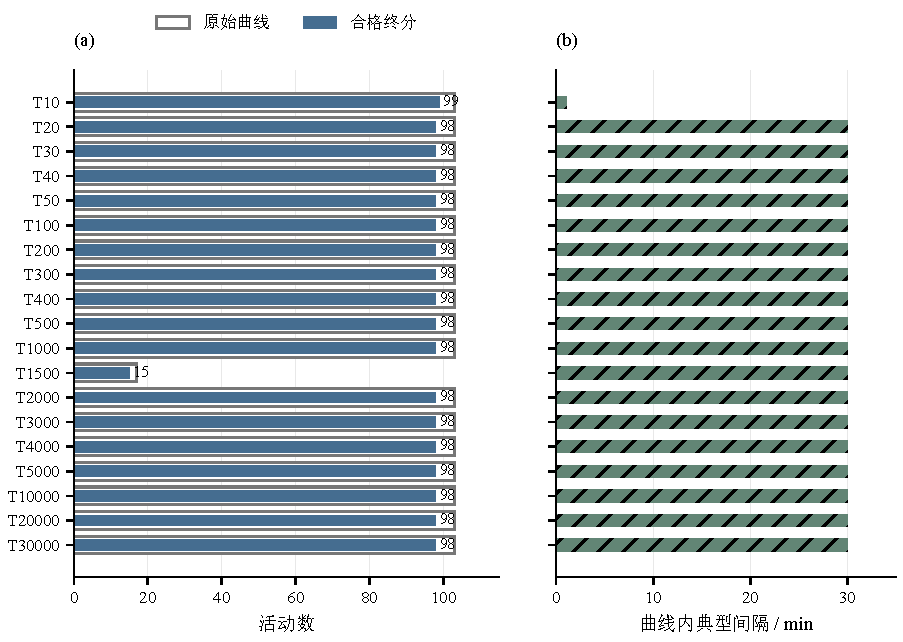
\includegraphics[width=\linewidth,height=.78\textheight,keepaspectratio]{figures/sampling_and_rank_coverage.pdf}
\caption{排名覆盖与采样分辨率。（a）原始曲线数和满足终点窗口的活动数；（b）曲线内典型观测间隔的跨活动中位数。T1500的来源覆盖较晚，所有排名均保留原始有效活动数。}
\label{fig:sampling}
\end{figure}

终分共同结构使用18条长期覆盖排名，另将T1500的成对可用结果完整导出。18线同时具有终分的活动为\NumCoreEvents{}期；要求半程也有合格观测后，为\NumCorrelationEvents{}期。分数增长另构建四条代表性排名的完整时间面板：T10、T1000、T2000和T30000在全部进度条件上共用\ProgressEvents{}期，在全部剩余时间条件上共用\RemainingEvents{}期。共同面板限制了缺测造成的直接混合，其结论适用于满足相应覆盖条件的活动\citep{rubin1976}。

\section{统计方法}

\subsection{分数分布、排名形状与时间比较}

对每条线报告终分中位数和四分位范围。以18线共同活动绘制排名与终分的对数坐标关系，描述同一活动集合的排名形状。跨年份比较固定为每年2月至10月，按国服实际开始日期归属年份，以减少首尾不完整月份造成的差异。各年活动数量、规则和乐队组成仍有变化，因此时间比较同时保留原始汇总与条件回归。

排名间的相对分数先在同一期计算，再跨活动汇总。例如：
\begin{equation}\label{eq:ratio}
R_e^{1000,2000}=\frac{Y_{e,1000}}{Y_{e,2000}}.
\end{equation}
比值中位数与两个边际中位数之比使用不同运算顺序，本文分别计算。年度比值区间采用2000次、长度为5期活动的循环移动块重采样，随机种子42\citep{kunsch1989}。块长度按活动计数，日历跨度随活动排程变化。

\subsection{活动进度与剩余增长}

在名义时刻\(t\)，取截至该时刻的末次观测\(u\leq t\)，要求至少有4个前缀观测，且\(t-u\leq60\ \mathrm{min}\)。定义分数占比和后续增长份额：
\begin{equation}\label{eq:growth}
F_{e,r}(t)=\frac{x_{e,r}(u)}{Y_{e,r}},\qquad
G_{e,r}(t)=1-F_{e,r}(t).
\end{equation}
进度条件为10\%、25\%、50\%、75\%、90\%和95\%；剩余时间条件为48、24、12、6、3、1、0.5和0.25小时。各条件保留实际观测时刻及滞后。“结束前6小时后增长”指该名义时刻之前末次观测至终分的增长，其实际覆盖时长还包含观测滞后。

为检查这一测量差异，补充分析仅对相邻观测间隔不超过60分钟的记录作线性插值，再与末次观测法逐案例比较。插值使用事后完整曲线，估计名义时刻的分数；该估计仅用于描述性敏感性分析。先在同一活动内平均各排名的份额差，再汇总活动中位数，避免高频采样或排名覆盖更多的活动取得更高权重。

\subsection{相关结构与主成分}

跨线关联采用Spearman相关\citep{spearman1904}。19线矩阵逐对使用共同活动，同时保存每格样本数。进一步在18线共同活动中计算秩变量的主成分：每条线的终分先转为秩，再中心化并标准化，最后作奇异值分解\citep{jolliffe2016}。方差比例描述排名分数的共同维度。

终分与半程剩余增长的比较严格使用相同的\NumCorrelationEvents{}期活动和153个线对。剩余增长变量为\(\log[Y_{e,r}/x_{e,r}(u_{0.5})]\)。条件调整秩相关先将各线终分转为秩，对活动时间、对数时长、类型与乐队哑变量作线性投影，再计算各线投影残差的Pearson相关。连续协变量保留上述模型形式，调整范围限于已列出的观测条件。

\subsection{活动条件的关联模型}

以所有合格活动和排名的对数终分为响应，拟合下式：
\begin{equation}\label{eq:association}
\begin{aligned}
\log Y_{e,r}&=\alpha_r+\beta\tau_e+\gamma\log D_e+
\theta_{k(e)}+\eta_{b(e)}+\varepsilon_{e,r},\\
\widehat{\symbf\beta}&=\arg\min_{\symbf b}
\sum_e\frac{1}{m_e}\sum_{r\in\mathcal R_e}
\bigl(\log Y_{e,r}-\symbf x_{e,r}^{\mathsf T}\symbf b\bigr)^2.
\end{aligned}
\end{equation}
其中\(D_e\)为活动小时数，\(\tau_e\)为自研究起点以来的年数，\(k(e)\)和\(b(e)\)为活动类型与乐队类别，\(m_e\)为该活动可用排名数。活动内各行权重为\(1/m_e\)，每期总权重相同。排名以T2000、类型以mission\_live、乐队以mixed为参照。主模型假定各排名共享时间、时长和活动条件系数。

标准误先以活动为单位汇总回归得分向量，避免把同一期的多条榜线视为独立观测\citep{cameron2015}。另采用Bartlett权重的5期HAC协方差\citep{newey1987}：
\begin{equation}\label{eq:hac}
\begin{aligned}
\widehat V&=cH^{-1}\!\left[\sum_es_es_e^{\mathsf T}
+\sum_{\ell=1}^{5}\left(1-\frac{\ell}{6}\right)
\sum_{e=\ell+1}^{G}
\bigl(s_es_{e-\ell}^{\mathsf T}+s_{e-\ell}s_e^{\mathsf T}\bigr)\right]H^{-1},\\
s_e&=\sum_rw_{e,r}\symbf x_{e,r}\widehat\varepsilon_{e,r},\quad
H=\sum_{e,r}w_{e,r}\symbf x_{e,r}\symbf x_{e,r}^{\mathsf T},\quad
c=\frac{G}{G-1}\frac{n-1}{n-k}.
\end{aligned}
\end{equation}
式中\(G\)为活动数、\(n\)为曲线行数、\(k\)为设计矩阵秩。活动按实际开始时间排序，使用\(G-1\)自由度的\(t\)与\(F\)近似。HAC以活动间隔而非固定日历时长度量相关；趋势与非平稳性仍可能影响区间近似。

因素的删项诊断定义为：
\begin{equation}\label{eq:partialr}
R^2_{\mathrm{partial},j}=
\frac{\mathrm{SSE}_{-j}-\mathrm{SSE}_{\mathrm{full}}}{\mathrm{SSE}_{-j}}.
\end{equation}
每个因素使用删去自身后的加权残差平方和作分母，分别比较。固定敏感性模型包含18线共同面板、二次时间项、近期卡牌上下文，以及T1000/T2000对数比。全部五个模型的\NumTests{}组因素检验统一作BY调整\citep{benjamini2001}。逐参数区间为边际区间，模型与检验均按探索性解释。补充材料另给出每次删除一期活动后的系数，检查个别活动的影响。

\subsection{内容元数据与角色暴露}

乐队类别由加成角色所属乐队确定：全部来自一个乐队时使用该乐队名称，多个乐队时标为mixed。角色暴露同时报告出现活动数，以及按同一期角色数量均分的活动权重：
\begin{equation}\label{eq:exposure}
W_c=\sum_{e:c\in\mathcal C_e}\frac{1}{|\mathcal C_e|}.
\end{equation}
该权重汇总为总活动数，描述内容排程中的角色出现。卡牌统计使用元数据国服发布时间，既报告研究末期已发布记录，也报告完整月份的新发布数量。关联扩展变量为活动开始前30天、与本期加成角色匹配的已发布卡牌数。玩家实际取得、培养及使用卡牌的情况未被观测。

\section{结果}

\subsection{排名分布与覆盖对汇总的影响}

18线共同终分面板保持了同一期内由较高名次到较低名次的分数顺序（图~\ref{fig:shape}a）。跨排名分数量级差异较大，对数坐标有助于同时展示T10至T30000。表~\ref{tab:ranks}提供全部19线的原量纲分布，并保留每档不同的活动数。

来源更新也会改变边际汇总。早期缓存中，T1000在97期活动的中位数为451.791万EP，T1500在14期的中位数为495.865万EP，出现跨档汇总倒序；这些活动内部的排名顺序保持一致。线上快照补全后，两档当前可用活动分别为98和15期，中位数变为448.074万与402.841万EP。在当前共同的\MatchedRareEvents{}期内，中位数为470.017万与402.841万EP。图~\ref{fig:shape}b同时展示三个口径。这一变化记录了样本更新与覆盖差异，分析排名形状时应使用相同活动集合。

\begin{figure}[!htbp]
\centering
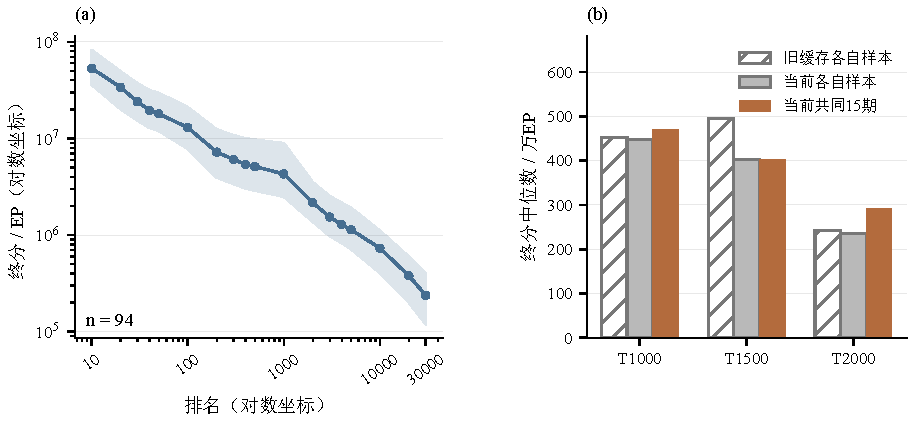
\includegraphics[width=\linewidth,height=.78\textheight,keepaspectratio]{figures/rank_shape_and_coverage_effect.pdf}
\caption{排名分数结构与覆盖口径。（a）\NumCoreEvents{}期共同活动的18线终分中位数及四分位范围；（b）旧缓存各自样本、当前各自样本及当前共同\MatchedRareEvents{}期的边际中位数。T1500未补造早期终分；三个口径的活动名单随补充数据提供。}
\label{fig:shape}
\end{figure}

\subsection{时间变化同时包含分数水平与排名形状}

相同月份比较显示，T1000终分中位数在2024、2025和2026年分别为261.509万、727.360万和642.136万EP；T2000为172.049万、270.305万和298.053万EP（表~\ref{tab:years}）。T1000在2025年较高，T2000在三年的中位数依次增加，不同榜线的变化方向和幅度存在差异。

\begin{table}[!htbp]
\centering\small
\caption{相同月份内的终分和排名比值}\label{tab:years}
\setlength{\tabcolsep}{4pt}
\renewcommand{\arraystretch}{1.15}
\begin{tabularx}{\linewidth}{l r r r r L}
\toprule
年份 & 活动数 & T1000 & T2000 & T30000 & T1000/T2000 \\
\midrule
2024 & 28 & 261.509 & 172.049 & 12.488 & 1.707 \\
2025 & 26 & 727.360 & 270.305 & 42.109 & 2.515 \\
2026 & 24 & 642.136 & 298.053 & 27.556 & 1.761 \\
\bottomrule
\end{tabularx}
\par\vspace{4pt}
\begin{minipage}{\linewidth}\footnotesize\setstretch{1.05}
注：各年均使用实际开始日期位于2月至10月的活动。三个终分列单位为万EP；比值列先对同活动两线相除，再汇总中位数。
\end{minipage}
\end{table}


在同活动配对后，T1000/T2000比值中位数为\RatioYearFirst{}、\RatioYearSecond{}和\RatioYearThird{}。图~\ref{fig:temporal}呈现逐活动比值和相同月份的块区间。2025年的比值较高，2026年回落；单一线性趋势难以概括这条序列。各年活动类型、乐队和时长组成同时变化，年度差异还需结合条件模型解释。

\begin{figure}[!htbp]
\centering
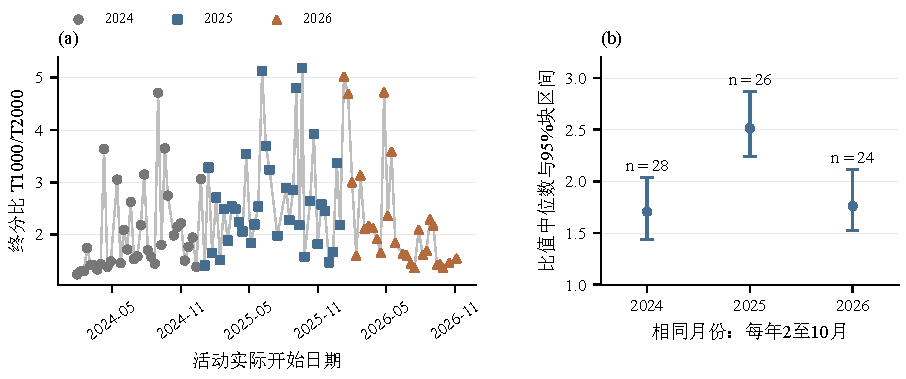
\includegraphics[width=\linewidth,height=.78\textheight,keepaspectratio]{figures/temporal_rank_ratio.pdf}
\caption{T1000/T2000终分比的时间变化。（a）全部成对可用活动，横轴为实际日历时间；（b）每年2月至10月的比值中位数与5活动循环块95\%区间，活动数依次为28、26和24。区间为探索性重采样描述。}
\label{fig:temporal}
\end{figure}

\subsection{T1000的末期增长份额高于代表性对照线}

共同进度面板中，半程已观测分数占终分的中位数，T10为\HalfTop{}\%，T1000为\HalfThousand{}\%，T2000为\HalfTwoThousand{}\%，T30000为\HalfThirtyThousand{}\%。共同剩余时间面板中，名义结束前6小时观测后的增长份额分别为\LateSixTop{}\%、\LateSixThousand{}\%、\LateSixTwoThousand{}\%和\LateSixThirtyThousand{}\%。T1000在这些活动中具有更高的末期增长占比（表~\ref{tab:growth}）。

\begin{table}[!htbp]
\centering\small
\caption{共同活动面板上的分数累积与后续增长}\label{tab:growth}
\setlength{\tabcolsep}{4pt}
\renewcommand{\arraystretch}{1.15}
\begin{tabularx}{\linewidth}{l *{4}{>{\centering\arraybackslash}X}}
\toprule
排名 & \shortstack{半程\\已观测 / \%} & \shortstack{90\%进度\\已观测 / \%} & \shortstack{结束前6h\\后续增长 / \%} & \shortstack{结束前1h\\后续增长 / \%} \\
\midrule
T10 & 68.053 & 98.247 & 0.218 & 0.000 \\
T1000 & 35.407 & 70.364 & 19.360 & 7.209 \\
T2000 & 48.063 & 82.166 & 11.790 & 6.060 \\
T30000 & 53.362 & 90.923 & 4.419 & 1.424 \\
\bottomrule
\end{tabularx}
\par\vspace{4pt}
\begin{minipage}{\linewidth}\footnotesize\setstretch{1.05}
注：进度面板为\ProgressEvents{}期，剩余时间面板为\RemainingEvents{}期；同一面板内四条线及所有时点共用活动。表中为活动中位数，后续增长相对终分归一化。
\end{minipage}
\end{table}


\begin{figure}[!htbp]
\centering
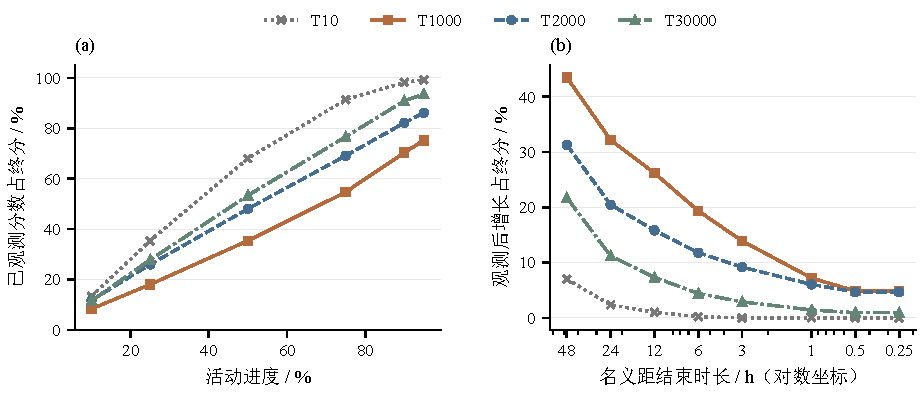
\includegraphics[width=\linewidth,height=.78\textheight,keepaspectratio]{figures/matched_rank_growth_profiles.pdf}
\caption{四条代表性排名的共同活动面板。（a）\ProgressEvents{}期在全部进度条件上的已观测分数比例；（b）\RemainingEvents{}期在全部剩余时间条件上的后续增长比例。曲线展示活动中位数；右图时间轴使用对数坐标并朝结束方向递减。各条件使用名义时刻前的末次观测，实际滞后另有记录。}
\label{fig:growth}
\end{figure}

不同排名的采样分辨率影响对末期增长的测量。补充线性插值检验中，名义结束前6小时的末次观测法比插值法得到更高的增长份额，逐活动平均差的中位数约为\InterpolationSix{}个百分点；结束前15分钟约为\InterpolationQuarter{}个百分点。短时距统计对时间对齐更敏感。分数增长的阶段差异有数据支持，榜线背后的玩家策略仍需个体记录检验。

\subsection{共同分数水平强于共同剩余增长}

18线共同终分的第一主成分解释\PcaFirst{}\%的标准化秩方差，前两个解释\PcaTwo{}\%。不同排名的终分存在较强共同变化。控制线性时间、对数时长、类型和乐队后的条件调整秩相关，中位数为\RhoPartial{}，低于未经条件调整的共同终分关联。

\begin{table}[!htbp]
\centering\small
\caption{终分与半程剩余增长的跨线关系}\label{tab:correlations}
\setlength{\tabcolsep}{4pt}
\renewcommand{\arraystretch}{1.15}
\begin{tabularx}{\linewidth}{L r r r r}
\toprule
分析对象 & 活动数 & 排名线 & 线对 & 中位相关 \\
\midrule
19线成对可用终分 & 12至98 & 19 & 171 & 0.912 \\
18线共同终分 & 94 & 18 & 153 & 0.912 \\
条件调整后的终分 & 94 & 18 & 153 & 0.736 \\
半程匹配面板的终分 & 92 & 18 & 153 & 0.915 \\
同面板半程剩余增长 & 92 & 18 & 153 & 0.471 \\
\bottomrule
\end{tabularx}
\par\vspace{4pt}
\begin{minipage}{\linewidth}\footnotesize\setstretch{1.05}
注：末两行严格使用同一批活动和线对。条件调整秩相关控制时间、时长、类型与乐队，具体投影形式见正文。
\end{minipage}
\end{table}


在相同的\NumCorrelationEvents{}期活动中，终分跨线相关中位数为\RhoFinal{}，半程剩余增长为\RhoGrowth{}（图~\ref{fig:correlations}）。两者使用相同活动、排名和线对，差异反映所分析变量不同。共同终分因子包含活动整体分数尺度；后续增长还具有排名和阶段对应的差异。主成分方差比例描述当前样本的共同结构，其预测用途需要另行评估。

\begin{figure}[!htbp]
\centering
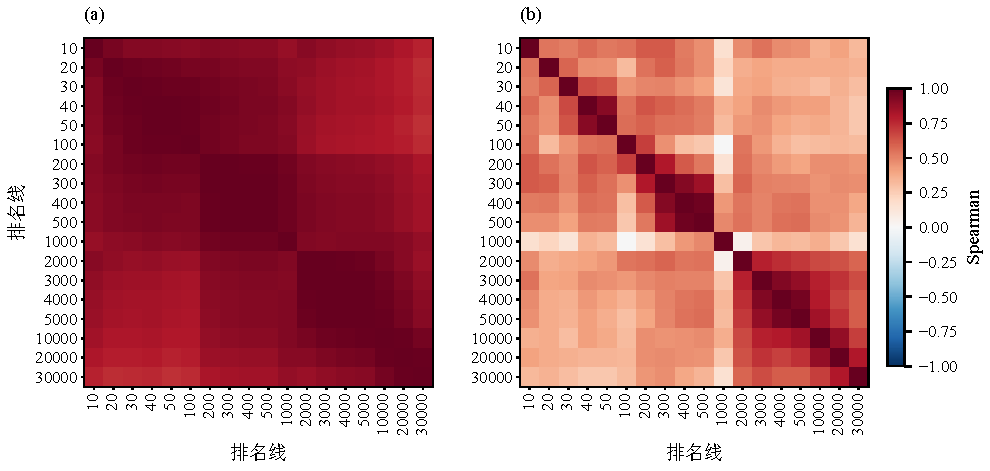
\includegraphics[width=\linewidth,height=.78\textheight,keepaspectratio]{figures/matched_score_growth_correlations.pdf}
\caption{同一\NumCorrelationEvents{}期活动、18线的Spearman相关。（a）最终分数；（b）半程剩余对数增长。两图共用色标，逐线对样本一致。T1500的成对结果在19线补充矩阵中提供。}
\label{fig:correlations}
\end{figure}

\subsection{活动类型与乐队具有条件分数关联}

主模型的时间项为\TimeBeta{}，5期HAC边际95\%区间为[\TimeLower{}，\TimeUpper{}]；对数时长系数为\DurationBeta{}，区间为[\DurationLower{}，\DurationUpper{}]。这些系数描述模型中其他变量给定时的活动间差异。模型允许各排名具有不同截距，并对活动类型和乐队作调整。

\begin{table}[!htbp]
\centering\small
\caption{主关联模型的删项诊断与整体检验}\label{tab:factors}
\setlength{\tabcolsep}{4pt}
\renewcommand{\arraystretch}{1.15}
\begin{tabularx}{\linewidth}{L r r L L}
\toprule
因素 & 自由度 & 偏$R^2$ & HAC检验$p$ & 全局BY调整$q$ \\
\midrule
排名 & 18 & 0.952 & $7.11\times10^{-118}$ & $2.38\times10^{-116}$ \\
活动类型 & 5 & 0.602 & $5.46\times10^{-40}$ & $9.12\times10^{-39}$ \\
乐队 & 8 & 0.339 & $1.53\times10^{-16}$ & $1.53\times10^{-15}$ \\
时间项 & 1 & 0.213 & $2.72\times10^{-8}$ & $1.61\times10^{-7}$ \\
活动时长 & 1 & 0.194 & $6.46\times10^{-9}$ & $4.32\times10^{-8}$ \\
\bottomrule
\end{tabularx}
\par\vspace{4pt}
\begin{minipage}{\linewidth}\footnotesize\setstretch{1.05}
注：偏$R^2$按删去该因素后的加权残差平方和定义。各因素的删项基准不同。BY调整覆盖五个固定模型中的全部\NumTests{}组因素检验。
\end{minipage}
\end{table}


在主模型的删项诊断中，排名、活动类型和乐队对应的偏\(R^2\)分别约为0.952、0.602和0.339。各项使用不同的删项基准，其数值分别解释。规则类型相对mission\_live的条件系数见图~\ref{fig:context}a；表~\ref{tab:bands}及图~\ref{fig:context}b报告乐队结果。

\begin{table}[!htbp]
\centering\small
\caption{乐队覆盖及终分的条件关联}\label{tab:bands}
\setlength{\tabcolsep}{4pt}
\renewcommand{\arraystretch}{1.15}
\begin{tabularx}{\linewidth}{L r r r C{4.4cm}}
\toprule
乐队类别 & 活动 & \shortstack{T1000\\有效活动} & \shortstack{T1000中位数\\/ 万EP} & 条件对数差 [95\%区间] \\
\midrule
mixed & 28 & 26 & 547.798 & 参照组 \\
Afterglow & 11 & 11 & 334.982 & 0.234 [0.093，0.375] \\
Hello, Happy World！ & 10 & 10 & 417.757 & 0.090 [−0.110，0.290] \\
Morfonica & 10 & 9 & 258.046 & 0.121 [−0.038，0.280] \\
Poppin'Party & 10 & 10 & 681.257 & 0.486 [0.306，0.666] \\
Roselia & 10 & 10 & 845.476 & 0.531 [0.345，0.717] \\
Pastel＊Palettes & 9 & 8 & 426.096 & 0.274 [0.105，0.444] \\
RAISE A SUILEN & 9 & 8 & 362.769 & 0.289 [0.051，0.526] \\
MyGO!!!!! & 6 & 6 & 2281.433 & 1.030 [0.707，1.352] \\
\bottomrule
\end{tabularx}
\par\vspace{4pt}
\begin{minipage}{\linewidth}\footnotesize\setstretch{1.05}
注：模型同时调整排名、时间、时长和活动类型，混合乐队为参照。区间为逐参数边际区间，采用按活动汇总得分向量的5期HAC估计。
\end{minipage}
\end{table}


MyGO!!!!!对应6期活动，其相对mixed的条件对数差为\MygoBeta{}，边际区间为[\MygoLower{}，\MygoUpper{}]。Poppin'Party和Roselia也具有正的条件分数差。每个乐队仅6至11期单乐队活动，系数仍依赖已有排程、规则分布和模型形式。补充的共同18线、二次时间及逐活动删除结果用于检查这些关联对样本和设定的敏感性。

\begin{figure}[!htbp]
\centering
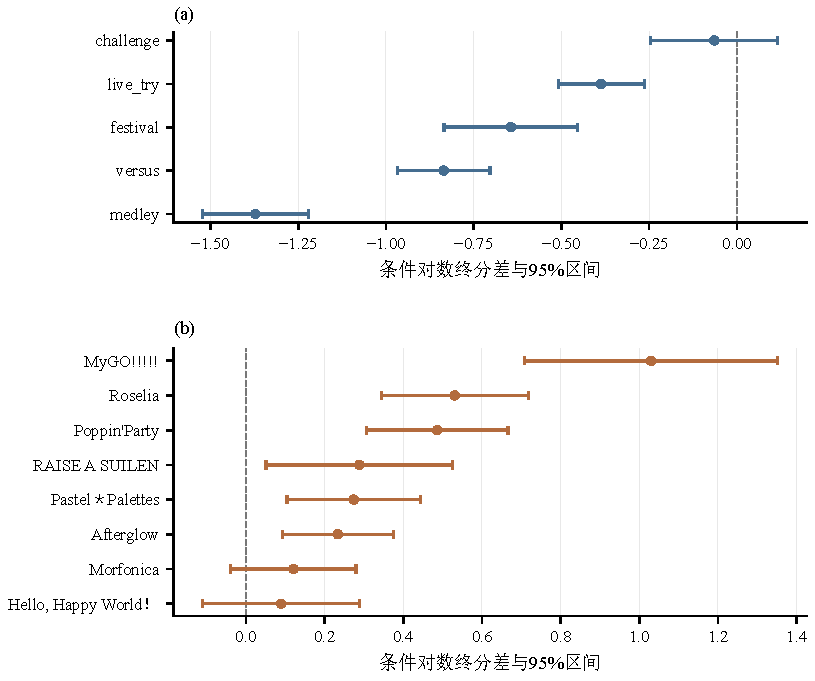
\includegraphics[width=\linewidth,height=.78\textheight,keepaspectratio]{figures/conditional_type_band_associations.pdf}
\caption{活动条件的回归系数与5期HAC边际95\%区间。（a）规则类型，以mission\_live为参照；（b）乐队，以mixed为参照。模型同时包含排名、时间与对数时长，系数表示条件对数终分差。}
\label{fig:context}
\end{figure}

\subsection{角色与卡牌记录描述内容供给}

103期活动共包含40位加成角色、\NumCharacterMemberships{}条角色与活动成员关系。角色出现次数与按式~\eqref{eq:exposure}计算的均分活动权重均随补充数据提供。单乐队活动75期，混合乐队28期；MyGO!!!!!为6期，其余单乐队类别为9至11期。图~\ref{fig:content}a展示全部40位角色的出现次数。

按元数据国服发布时间过滤，在最后一场研究活动开始时，缓存中有\NumCards{}条已发布卡牌记录，其中\NumFiveStar{}条为5星。图~\ref{fig:content}b仅使用2024年2月至2026年10月的完整月份，描述新发布卡牌的记录数量。该统计反映元数据中的内容供给，角色受欢迎程度和玩家持卡分布需要另外测量。

\begin{figure}[!htbp]
\centering
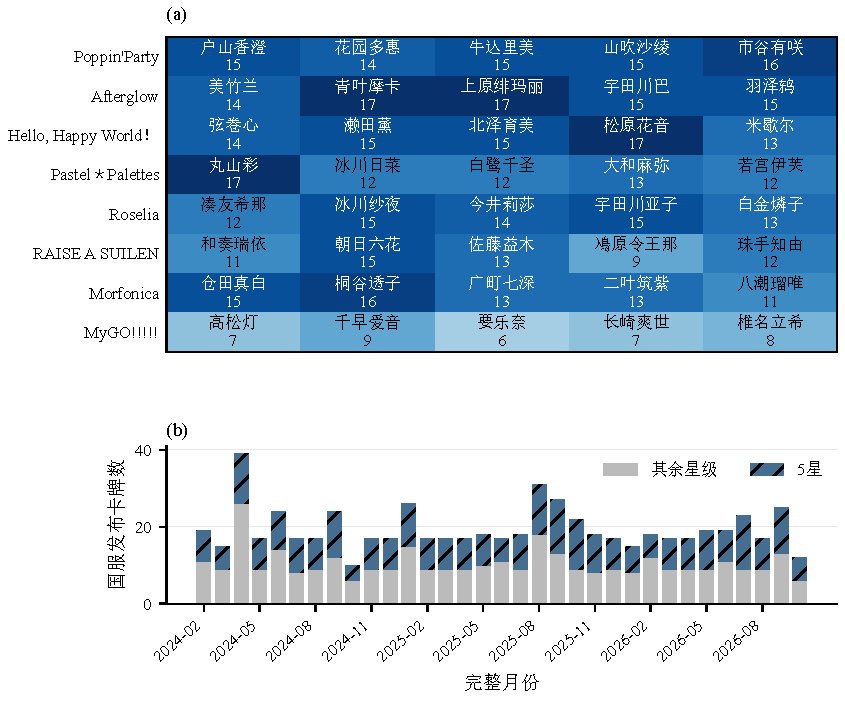
\includegraphics[width=\linewidth,height=.78\textheight,keepaspectratio]{figures/character_exposure_and_card_releases.pdf}
\caption{活动角色与卡牌发布记录。（a）全部40位加成角色在103期活动中的出现次数，按乐队和角色ID排列；（b）完整月份的国服卡牌发布记录，按5星与其他星级分组。出现次数采用每期角色成员关系计数，未使用玩家选择或购买数据。}
\label{fig:content}
\end{figure}

加入活动开始前30天、与加成角色匹配的卡牌发布数量后，该变量系数为\CardBeta{}，HAC区间为[\CardLower{}，\CardUpper{}]，全局BY调整后\(q=1\)。当前模型对这一变量的独立关联估计不精确。卡牌发布、玩家持有和实际加成使用属于不同观测层次，后续需要取得持卡与使用信息再检验其作用。

\FloatBarrier
\section{讨论}

\subsection{分数尺度、排名形状和增长过程应分别描述}

共同终分的低维结构与排名比值的时间变化同时存在。前者说明多条榜线随活动背景共同变化，后者说明活动内部的分数形状仍会改变。T1000/T2000在2025年较高、2026年回落，而T2000的同月终分中位数继续增加，显示共同尺度与局部比例具有不同的变化方式。

阶段增长也有排名差异。T10在共同面板的半程累积比例较高，T1000在末期仍有较大的后续增长。依据汇总榜线，可以描述这些分数变化发生的位置和幅度；判断其是否源于奖励门槛、集中游玩或特定策略，需要玩家行为及计分机制的额外记录。对游戏活动的统计描述应同时提供原量纲水平、相对排名比和归一化增长，避免由单个指标概括整个活动。

\subsection{测量与覆盖会改变可见模式}

T10高频采样与其他档位较低频采样共同存在，密集采样时期仍有档位间的分辨率差异。对末期15分钟之类的短窗口，末次观测与名义时刻的距离会占据较大比例。记录滞后、使用相同活动及补充插值敏感性，可以帮助区分采样造成的差异和曲线本身的差异。

T1500的缓存更新展示了另一类测量问题：少量新增活动就能改变小样本的中位数和跨档排序。当前相同活动的排名顺序保持一致，而边际中位数随活动组成变化。公开数据分析应将更新版本、有效活动数和比较名单作为统计量的组成部分，与数值一并保存。

\subsection{条件关联与解释范围}

活动类型和乐队与终分具有条件关联，说明只按年份或单一榜线描述分数还会遗漏结构。规则类型可能同时对应计分机会、参与条件和活动内容，乐队也与排程及主题绑定。回归控制了已记录变量，其他共同变化仍可能留在系数中。若要估计更换乐队或调整规则的干预效果，需要明确识别条件与对照设计\citep{hernan2020}。

MyGO!!!!!的条件系数来自6期活动，适合继续核查具体活动组成。近期匹配角色卡牌发布数量的区间跨零，也提示发布数量这一代理量与玩家实际可用资源之间仍有距离。后续内容研究可以在保留聚合统计的基础上，接入可合法使用的持卡、实际加成、游玩与奖励获得记录，检验这些解释所需的观测链条。

\subsection{局限与可复核性}

样本来自一个游戏、一个服务器及指定时期，外部适用性有待其他场景检验。部分活动此前已参与预测模型探索，验证活动曾被反复使用；本文的全样本关联分析按探索性解释。活动、角色及卡牌元数据为回溯快照，历史时点档案的缺失会影响当时内容可用状态的重建。

共同面板减少覆盖组成的直接差异，也可能选择记录较完整的活动。19线逐对矩阵、18线共同矩阵和T1500小样本各有不同的有效总体，结果分别保存。活动内多排名依赖由聚类方法处理，活动间趋势和不规则排程仍会影响HAC与移动块近似。BY调整处理预先列出的因素检验，回归系数区间仍为边际区间，未覆盖所有潜在分析选择。

终分窗内的最后记录是本研究的测量定义，后续榜单修订可能产生不同值。分数下降与负增长记录均保留，来源更新通过独立快照追踪。全部统计脚本、活动名单、排除原因、矩阵支持数和表图输入均随稿提供，读者可以据此检查特定时点、排名或活动条件对应的结论。

\Needspace{9\baselineskip}
\section{结论}

本文整理了\NumEvents{}期国服活动、19档排名的只读快照，得到\NumValidCurves{}条满足终点窗口的曲线。相同活动内的终分具有较强共同结构，而半程剩余增长的跨线关联较弱；T1000在代表性共同面板中具有较高的末期增长份额。T1000/T2000比值在相同月份的年度中位数呈非单调变化，活动类型与乐队在控制排名、时间和时长后仍与终分相关。

公开榜线的解释依赖终点定义、实际观测时刻和活动覆盖。角色出现与卡牌发布记录补充了内容排程信息，玩家规模、偏好和个体资源使用仍需其他数据测量。上述结果为后续游戏活动研究提供了可复核的分数结构、阶段增长和活动条件描述。

\FloatBarrier
\section*{数据与代码可用性}

原始来源为Bestdori公开数据\citep{bestdori2026}。随稿材料包含2026年11月18日的只读数据快照、103期活动名单、19线覆盖、分时点数据、条件模型及敏感性结果，并提供表图生成与独立核验脚本。主快照的规范化记录SHA-256前12位为\texttt{\SourceFingerprint{}}，完整指纹及来源文件哈希见\texttt{data/source\_manifest.json}。早期缓存的核查数据另附来源标记。

研究代码入口为\href{https://github.com/AhsokaTano26/BanG-DreamActivity-fraction-prediction/tree/research/innovation-20261113}{BanG Dream Activity fraction prediction}。精确稿件版本以本地随稿清单及文件指纹确定，公开分支与本地材料的发布状态在说明文件中分别记录。

\section*{生成式人工智能使用声明}

本文使用OpenAI的ChatGPT和Codex辅助制定统计定义、编写与执行分析代码、检查数据、生成图表、编排LaTeX及修改语言。统计量由随稿脚本在来源快照上计算，表格和正文数值采用统一绑定。署名作者负责审核研究内容并确认投稿版本。

\begingroup\raggedright\small
\bibliographystyle{elsarticle-num}
\bibliography{references}
\endgroup
\end{document}
